%%%%%%%%% BODY TEXT
\section{Introduction}

The objective of multiple object tracking is to find a trajectory for each individual object of interest in a given input video. 
Specific interest has been devoted to the specific task of multiple person tracking~\cite{zamir2012gmcp,henschel2017improvements,tang2016multi,tang2017multiple,luo2014multiple}. 
Most successful approaches follow the \textit{Tracking-By-Detection} paradigm.
First, an object (pedestrian) detector is used in order to retrieve the position of each person within each frame. 
Secondly, the output detections of same persons across video frames are associated over space and time in order to form unique trajectories. 
Since objects might get occluded during the video sequence or the detector might simply fail on some examples, successful approaches are usually based not solely on spatial but also on appearance cues. These are learned from annotated data, for example using Siamese networks for person re-identification~\cite{tang2017multiple}.\\

\begin{figure}[t]
	\begin{center}
		%\fbox{\rule{0pt}{2in} \rule{0.9\linewidth}{0pt}}
		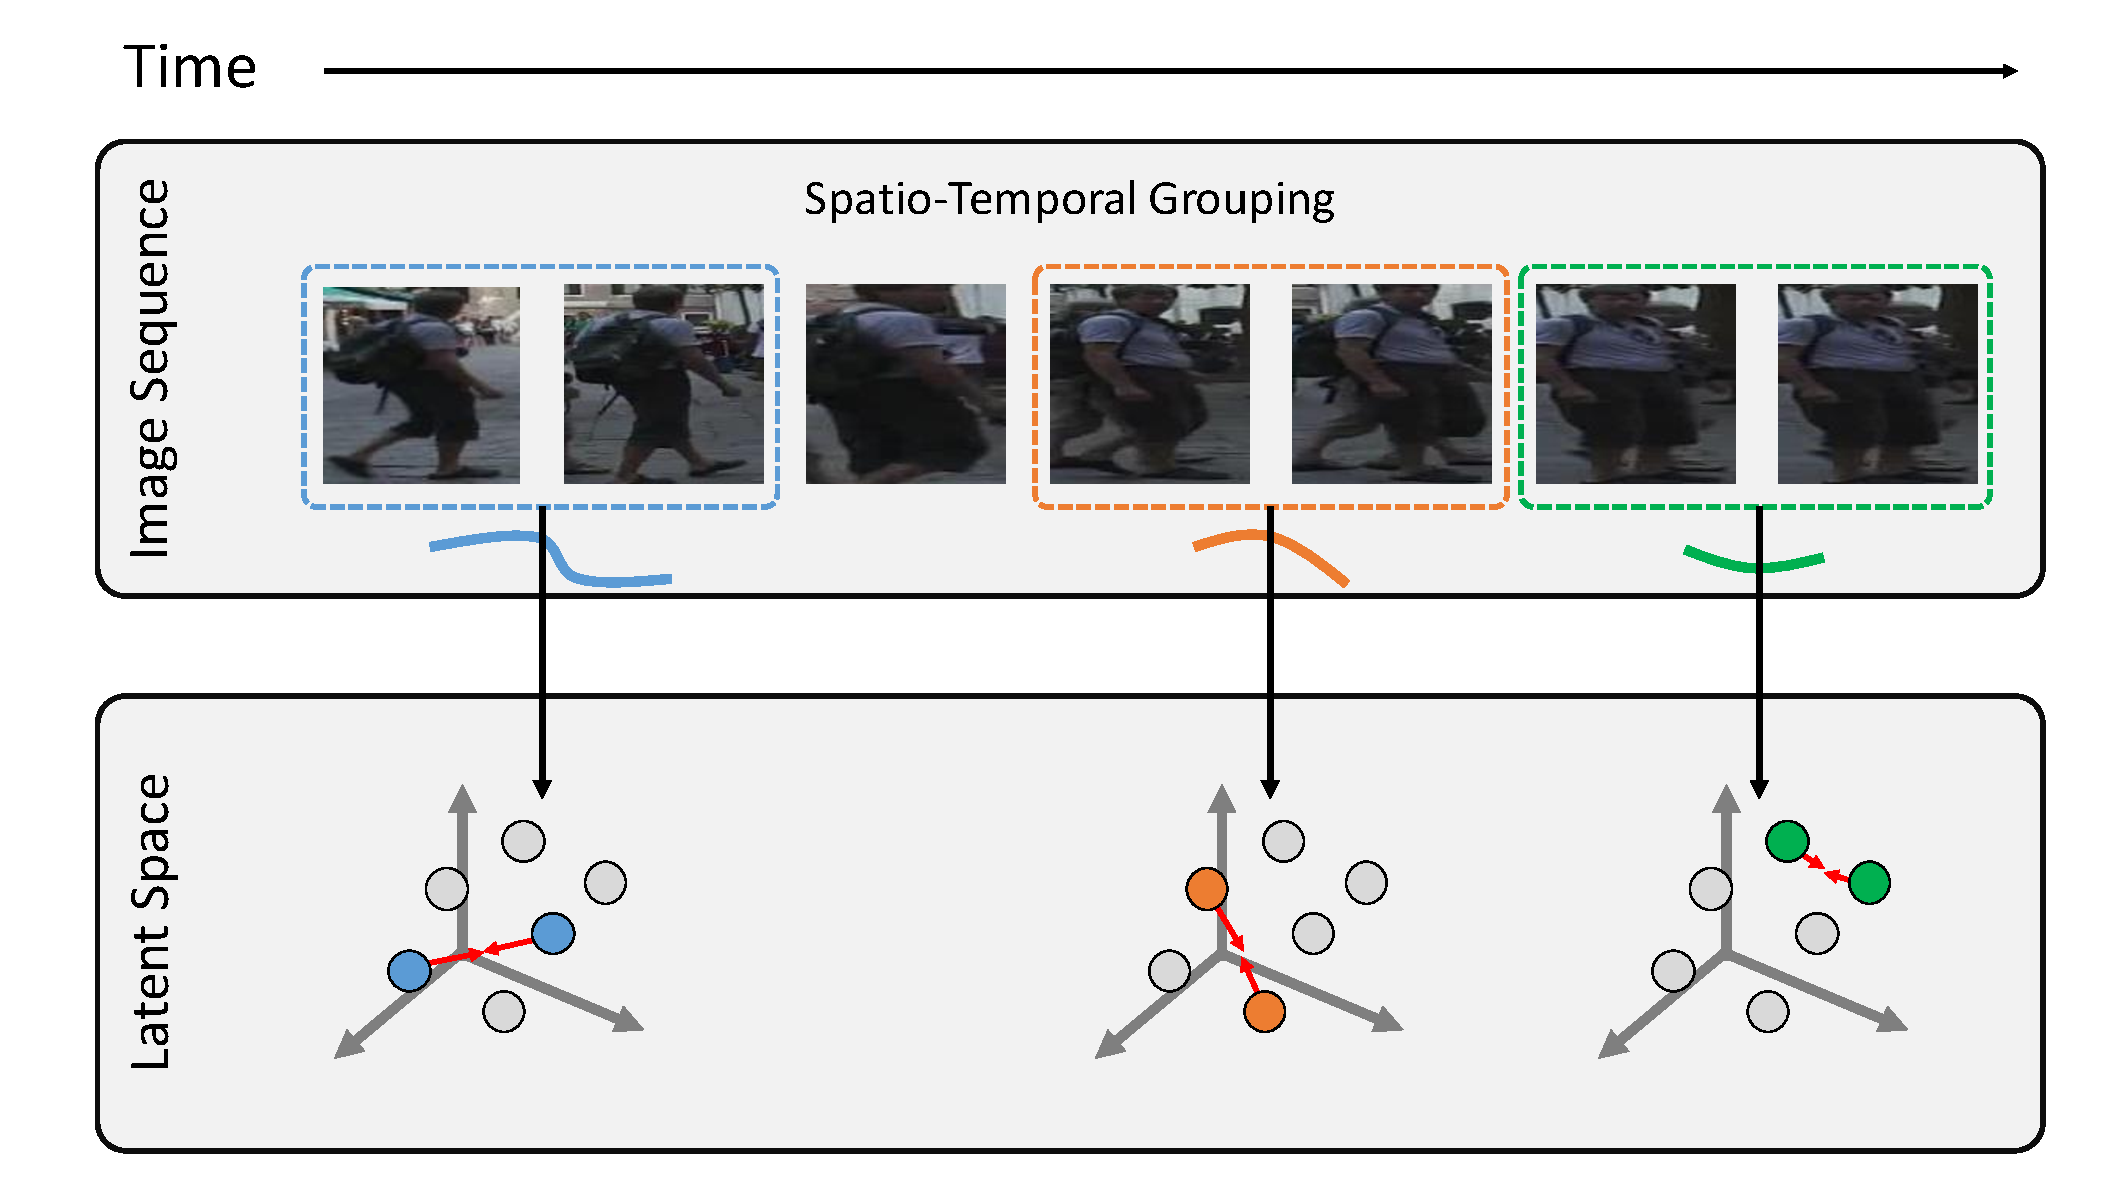
\includegraphics[width=0.7\linewidth]{Fig_1_teaser.pdf}
	\end{center}
	%\caption{Visualization of the proposed idea: a) Appearance centroid from spatio-temporal information. b) The appearance space is trained to minimize the distance between centroid and associated detections.}
	\caption{Given an image sequence, many data associations can be made reliably from pure spatio-temporal cues such as the intersection over union of bounding boxes. These associations are injected into a convolutional AutoEncoder to enforce detections with the same, spatio-temporally determined label to be close to one-another in the latent space. Thus, the learned appearance features will generalize over viewpoint and pose variations.}
	\label{fig:teaser}
\vspace*{-5mm}
\end{figure}
\noindent\textbf{Motivation.}
Supervised approaches for person re-identification require large amounts of sequence specific data in order to achieve good performance. For this reason, multiple object tracking benchmarks such as MOT~\cite{MOT16} are providing a training  sequence recorded in a sufficiently similar setting for every test sequence. The results of our experiments in table \ref{tab:supervised_compare} confirm this dependency and show the high variance in the quality of supervised approaches, depending on the data used for training. The standard approach to solve this problem is to incorporate additional annotated training data. For example, \cite{yoon2018online, feng2019multi} showed that additional data is key to improving the overall tracking performance.



Thus, publicly available, annotated training data currently seems not to be sufficient for training reliable person re-identification networks. Furthermore, recording and labeling sufficient data in a setting close to a final test scenario usually comes at a high price. Hence, the need for methods with a low amount of supervision becomes obvious and motivates us to propose a multiple object tracking method based on self-supervision.\\
While self-supervised learning methods~\cite{kolesnikov2019revisiting} have been successfully exploited in other vision tasks~\cite{watch_move,mahendran2018cross,hendrycks2019using,self_pedest,bb_annot,col_vid}, a direct application to tracking is non-trivial: Learning suitable object appearance metrics for object tracking in a self-supervised way is challenging since, compared to classical clustering problems, visual features of the same person may change over time due to pose and viewpoint changes and partial occlusion.
Other issues, such as frequent and long range full occlusion or background noises, makes pedestrian tracking even more challenging.\\

%Recently, Deep Neural Networks (DNN) have gained significant role in research and industry. DNN enables ``learning from data'', therefore it is often used when a significant large amount of data is available where the goal is to find patterns or features in it. 
%By extracting these features, one can build a model to correctly classify unseen data if the correct labels are provided. 
%This is called supervised learning. 
%On the other hand, unsupervised approaches group similar data together into clusters.
%This is often more challenging as the model has to associate the correct data together without any ground truth. 
%Self-supervised approaches however use unlabelled data to formulate a pretext task, where the objective can be derived without supervision~\cite{kolesnikov2019revisiting}.

In this paper, we propose an approach for learning appearance features for multiple object tracking without utilizing human annotations of the data. 
Our approach is based on two observations:  I) given an image sequence, many data associations can be made reliably from pure spatio-temporal cues such as the intersection over union (IoU) of bounding boxes within one frame or between neighboring frames. 
II) Resulting tracklets, carry important information about the variation of an object's appearance over time, for example by changes of the pose or viewpoint. 
In our model, we cluster the initial data based on simple spatial cues using the recently successful minimum cost multicut approach \cite{tang2016multi}. 
The resulting clustering information is then injected into a convolutional AutoEncoder to enforce detections with the same, spatio-temporally determined label to be close to one-another in the latent space (see Fig.\ref{fig:teaser}). 
Thus, the resulting latent data representation is encoding not only the pure object appearance, but also the expected appearance variations within one object ID. 
Distances between such latent representations can serve to re-identify objects even after long temporal distances, where no reliable spatio-temporal cues could be extracted. 
We use the resulting information in the minimum cost lifted multicut framework, similar to the formulation of Tang~\cite{tang2017multiple}, whose method is based on Siamese networks trained in a fully supervised way. To summarize, our contributions are:
\begin{itemize}
    \item We present an approach for multiple object tracking, including long range connections between objects, which is completely supervision-free in the sense that no human annotations of person IDs are employed.
	\item We propose to inject spatio-temporally derived information into convolutional AutoEncoder in order to produce a suitable data embedding space for multiple object tracking.
	\item  We evaluate our approach on the challenging MOT17 benchmark and show competitive results without using training annotations. 
\end{itemize}
\begin{table}[t]
	\begin{center}
	{
    \scriptsize
		\offinterlineskip
		\hspace*{3mm}
		\hspace*{0.9cm}\MyHBox{02}\MyHBox{04}\MyHBox{05}\MyHBox{09}\MyHBox{10}\MyHBox{11}\MyHBox{13}\par
        \vspace{-0.2cm}
		\MyTBox{02}{\textbf{100}}{\textcolor{c_red}{-0.3}}{\textcolor{c_red}{-0.6}}{\textcolor{c_red}{-11.9}}{\textcolor{c_red}{-11.9}}{\textcolor{c_red}{-9.8}}{\textcolor{c_red}{-14.0}}
		\MyTBox{04}{0.0}{\textbf{100}}{0.0}{\textcolor{c_red}{-11.6}}{\textcolor{c_red}{-11.6}}{\textcolor{c_red}{-4.9}}{\textcolor{c_red}{-9.5}}
		\MyTBox{05}{\textcolor{c_red}{-0.2}}{\textcolor{c_red}{-0.6}}{\textbf{100.0}}{\textcolor{c_red}{-2.0}}{\textcolor{c_red}{-2.0}}{\textcolor{c_red}{-5.1}}{\textcolor{c_red}{-3.6}}
		\MyTBox{09}{0.0}{\textcolor{c_red}{-0.2}}{0.0}{\textbf{100.0}}{0.0}{\textcolor{c_red}{-2.2}}{\textcolor{c_red}{-0.5}}
		\MyTBox{10}{0.0}{\textcolor{c_red}{-0.4}}{\textcolor{c_green}{0.2}}{0.0}{\textbf{100.0}}{\textcolor{c_red}{-0.8}}{\textcolor{c_green}{0.4}}
		\MyTBox{11}{\textcolor{c_green}{0.9}}{\textcolor{c_green}{0.9}}{\textcolor{c_green}{1.0}}{\textcolor{c_green}{1.6}}{\textcolor{c_green}{1.6}}{\textbf{100.0}}{\textcolor{c_green}{1.0}}
		\MyTBox{13}{\textcolor{c_green}{2.2}}{\textcolor{c_green}{2.2}}{\textcolor{c_green}{2.2}}{\textcolor{c_green}{0.2}}{\textcolor{c_green}{0.2}}{\textcolor{c_green}{1.3}}{\textbf{100.0}}
	}
	\vspace*{5mm}
	\caption{
	Results for training with one training sequence using \emph{GT annotations}\footnotemark for the tracklet generation, and evaluating on another training sequences with different viewpoints and resolutions. 
%Specifically, we mine GT tracklets from the detections with IoU $>0.5$ with the GT as e.g. done in~\cite{leal2016learning}.
%Tab. \ref{tab:supervised_compare} shows the results in terms of decay in performance when non-matching sequences are used for training.
	this table shows the relative MOTA changes for non-matching sequences on MOT17, FRCNN in comparison to the baseline (bold). Columns represent the training sequence, rows the test sequence. Cross-sequence tracking performance is unstable.
}
	\vspace*{-5mm}
	\label{tab:supervised_compare}
	\end{center}
\end{table}
The rest of the paper is structured as follows. \footnotetext{ 
Specifically, we mine GT tracklets from the detections with IoU $>0.5$ with the GT as e.g. done in~\cite{leal2016learning}.}
Section \ref{sec:related} discusses the related work on multiple object tracking. 
Our self-supervised approach on multiple object tracking is explained in Section \ref{subsec:method}. 
In Section \ref{sec:results}, we show the tracking performance of the proposed method in the MOT Benchmark ~\cite{MOT16} and conclude in  %\footnote{\url{https://motchallenge.net/data/MOT17/}}. 
%A conclusion is summarized 
 Section \ref{sec:conclusion}.



